\documentclass[11pt]{article}

% packages
\usepackage{physics}
% margin spacing
\usepackage[top=1in, bottom=1in, left=0.5in, right=0.5in]{geometry}
\usepackage{hanging}
\usepackage{amsfonts, amsmath, amssymb, amsthm}
\usepackage{systeme}
\usepackage[none]{hyphenat}
\usepackage{fancyhdr}
\usepackage[nottoc, notlot, notlof]{tocbibind}
\usepackage{graphicx}
\graphicspath{{./images/}}
\usepackage{float}
\usepackage{siunitx}
\usepackage{esint}
\usepackage{cancel}

% header/footer formatting
\pagestyle{fancy}
\fancyhead{}
\fancyfoot{}
\fancyhead[L]{MAS4105 Dr. Zhang}
\fancyhead[C]{HW9}
\fancyhead[R]{Sai Sivakumar}
\fancyfoot[R]{\thepage}
\renewcommand{\headrulewidth}{0pt}

% paragraph indentation/spacing
\setlength{\parindent}{0cm}
\setlength{\parskip}{5pt}
\renewcommand{\baselinestretch}{1.25}

% extra commands defined here
\newcommand{\ihat}{\boldsymbol{\hat{\textbf{\i}}}}
\newcommand{\jhat}{\boldsymbol{\hat{\textbf{\j}}}}
\newcommand{\dr}{\vec{r}~^{\prime}(t)}
\newcommand{\dx}{x^{\prime}(t)}
\newcommand{\dy}{y^{\prime}(t)}

\newcommand{\br}[1]{\left(#1\right)}
\newcommand{\sbr}[1]{\left[#1\right]}
\newcommand{\cbr}[1]{\{#1\}}

\newcommand{\dprime}{\prime\prime}
\newcommand{\lap}[2]{\mathcal{L}[#1](#2)}

% bracket notation for inner product
\usepackage{mathtools}

\DeclarePairedDelimiterX{\abr}[1]{\langle}{\rangle}{#1}

\DeclareMathOperator{\Span}{span}
\DeclareMathOperator{\nullity}{nullity}

% set page count index to begin from 1
\setcounter{page}{1}

\begin{document}

2.4: 2(c), 15, 16, 17, 20\\

2. Determine whether $\mathsf{T}$ is invertible or not.

(c) The transformation is invertible. To prove this, we must show that $\mathsf{T}$ is injective and surjective (bijectivity is equivalent to invertibility).

Injectivity. We may show this by showing the nullspace consists of only the zero vector, that is, the only vector that maps into the zero vector will be the zero vector itself. 

The following system of equations and its solution (obtained through elimination) \begin{equation*}
    \sysdelim..\systeme{
    3a_1 -2a_3 = 0,
    a_2 = 0,
    3a_1 + 4a_2 = 0 
    }\to
    \sysdelim..\systeme{
    a_1 = 0,
    a_2 = 0,
    a_3 = 0
    }
\end{equation*} indicates that the only vector $(a_1,a_2,a_3)$ that will map into the zero vector is the zero vector itself, so the nullspace contains only the zero vector and so $\mathsf{T}$ is injective.

Surjectivity. We must show that for some arbitrary vector $(A,B,C)$, there exists a vector $(a,b,c)$ such that $\mathsf{T}(a,b,c) = (A,B,C)$.

This then reduces to finding the solution to the following system of equations:
\begin{equation*}
    \sysdelim..\systeme{
    3a_1 -2a_3 = A,
    a_2 = B,
    3a_1 + 4a_2 = C 
    }
\end{equation*} The solution is (via elimination)
\begin{align*}
    a_1 &= \frac{C-4B}{3}\\
    a_2 &= B\\
    a_3 &= \frac{C-4B-A}{2}.
\end{align*}

Because the system is not inconsistent (we have an actual solution), we have the vector $(a,b,c)$ we desire. Thus $\mathsf{T}$ is surjective, and so $\mathsf{T}$ is bijective and hence invertible.

15. Let $\mathsf{V}$ and $\mathsf{W}$ be finite-dimensional vector spaces, and let $\mathsf{T} : \mathsf{V} \to \mathsf{W}$ be a linear transformation. Suppose that $\beta$ is a basis for $\mathsf{V}$. Prove that $\mathsf{T}$ is an isomorphism if and only if $\mathsf{T}(\beta)$ is a basis for $\mathsf{W}$.

\begin{proof}
    Forwards direction. Suppose $\mathsf{T}(\beta)$ is a basis for $\mathsf{W}$. Since $\mathsf{T}(\beta)$ is a basis, we know that $\mathsf{T}(\beta)$ is linearly independent, and so from a previous result that if $\mathsf{T}$ maps linearly independent subsets of $\mathsf{V}$ to linearly independence subsets of $\mathsf{W}$, then $\mathsf{T}$ is injective. So $\mathsf{T}$ is injective.

    What remains is to show that $\mathsf{T}$ is surjective. Since $\mathsf{T}$ is linear we need not worry about the zero vector in $\mathsf{W}$ having a preimage in $\mathsf{V}$. So for any nonzero vector $w\in\mathsf{W}$, we must find a (known to be nonzero) vector $v\in\mathsf{V}$ such that $\mathsf{T}(v) = w$.

    We can express $w$ as a linear combination of vectors in $\mathsf{T}(\beta)$. Let $\beta = \cbr{v_1,v_2,\dots,v_n}$ and $\mathsf{T}(\beta) = \cbr{w_1,w_2,\dots,w_n}$, where $w_i = \mathsf{T}(v_i)$ (there are $n$ vectors in both sets since $\mathsf{T}$ is injective). Then $w = c_1w_1 + c_2w_2 + \cdots + c_nw_n$ for scalars $c_i$, since $\mathsf{T}(\beta)$ is a basis. Then $w = c_1\mathsf{T}(v_1) + c_2\mathsf{T}(v_2) + \cdots + c_n\mathsf{T}(v_n) = \mathsf{T}(c_1v_1 + c_2v_2 + \cdots + c_nv_n)$, so we have that $v = c_1v_1 + c_2v_2 + \cdots + c_nv_n$, which means that $\mathsf{T}$ is indeed surjective.

    Since $\mathsf{T}$ is bijective, then it is invertible and thus $\mathsf{T}$ is an isomorphism.

    Converse. Let $\mathsf{T}$ be an isomorphism. Then since $\mathsf{T}$ is injective, we know that $\mathsf{T}(\beta)$ will be a linearly independent subset of $\mathsf{W}$. Again, let $\beta = \cbr{v_1,v_2,\dots,v_n}$ and $\mathsf{T}(\beta) = \cbr{w_1,w_2,\dots,w_n}$, where $w_i = \mathsf{T}(v_i)$ (there are $n$ vectors in both sets since $\mathsf{T}$ is injective).

    To show that $\mathsf{T}(\beta)$ generates $\mathsf{W}$, consider by way of contradiction that $\mathsf{T}(\beta)$ does not generate $\mathsf{W}$. Then we may extend $\mathsf{T}(\beta)$ by way of the replacement theorem into a basis for $\mathsf{W}$. Then a basis for $\mathsf{W}$ can be $\gamma = \cbr{w_1,w_2,\dots,w_n, W_1, W_2, \dots, W_m}$, where each $W_i\in\mathsf{W}$ was chosen in a way to retain the linear independence of $\gamma$ and finally have $\gamma$ be a generator for $\mathsf{W}$.

    But $\mathsf{T}$ is surjective (and linear), so for each of the $W_i$, we have that $W_i = \mathsf{T}(c_{i1}v_1 + c_{i2}v_2 + \cdots + c_{in}v_n) = c_{i1}\mathsf{T}(v_1) + c_{i2}\mathsf{T}(v_2) + \cdots + c_{in}\mathsf{T}(v_n) = c_{i1}w_1 + c_{i2}w_2 + \cdots + c_{in}w_n$. Hence $\gamma$ is not linearly independent, which is a contradiction. 
    
    Therefore there was no need to extend $\mathsf{T}(\beta)$ into a basis for $\mathsf{W}$ and so $\mathsf{T}(\beta)$ is a basis for $\mathsf{W}$.

    Hence $\mathsf{T}$ is an isomorphism if and only if $\mathsf{T}(\beta)$ is a basis for $\mathsf{W}$.
\end{proof}

16. Let $B$ be an $n\times n$ invertible matrix. Define $\Phi : \mathsf{M}_{n\times n}(\mathbb{F})\to \mathsf{M}_{n\times n}(\mathbb{F})$ by $\Phi(A) = B^{-1}AB$. Prove that $\Phi$ is an isomorphism.

\begin{proof}
    It is sufficient to show that $\Phi$ is bijective, i.e. invertible.

    Injectivity. We must show that for two $n\times n$ matrices $A$ and $C$, if $\Phi(A) = \Phi(C)$, then $A=C$. So $\Phi(A) = B^{-1}AB = B^{-1}CB = \Phi(C)$. Then by left and right multiplication we can do $B(B^{-1}AB)B^{-1} = B(B^{-1}CB)B^{-1}$. But $\mathsf{M}_{n\times n}(\mathbb{F})$ is a group under matrix multiplication, so we have associativity. Then $(BB^{-1})A(BB^{-1}) = (BB^{-1})C(BB^{-1}) = IAI = ICI = A = C$. Thus $\Phi$ is injective.

    Surjectivity. We must show that for some $n\times n$ matrix $C$, there is another $n\times n$ matrix $A$ such that $C = \Phi(A) = B^{-1}AB$. Like before, do a left and right multiplication and use the associativity property, so $BCB^{-1} = (BB^{-1})A(BB^{-1}) = IAI = A$. Since $BCB^{-1} \in \mathsf{M}_{n\times n}(\mathbb{F})$, then we have that $\Phi$ is indeed surjective.

    Thus $\Phi$ is bijective and so invertible, and so $\Phi$ is an isomorphism.
\end{proof}

17.$^\dagger$ Let $\mathsf{V}$ and $\mathsf{W}$ be finite-dimensional vector spaces and $\mathsf{T} : \mathsf{V} \to \mathsf{W}$ be an isomorphism. Let $\mathsf{V}_0$ be a subspace of $\mathsf{V}$.

(a) Prove that $\mathsf{T}(\mathsf{V}_0)$ is a subspace of $\mathsf{W}$.

\begin{proof}
    We must show that $\mathsf{T}(\mathsf{V}_0)$ contains the zero vector of $\mathsf{W}$, is closed under vector addition, and is closed under scalar multiplication. 

    Since $\mathsf{T}$ is an isomorphism, it is linear and so the zero vector of $\mathsf{V}_0$ maps to the zero vector of $\mathsf{W}$, so $\mathsf{T}(\mathsf{V}_0)$ contains the zero vector of $\mathsf{W}$.

    Take two vectors $w_1,w_2\in \mathsf{T}(\mathsf{V}_0)$, where $w_1 = \mathsf{T}(a_1v_1+a_2v_2+\cdots + a_nv_n)$ and $w_2 = \mathsf{T}(b_1v_1+b_2v_2+\cdots + b_nv_n)$ Each $v_i$ is in $\mathsf{V}_0$, and each $a_i,b_i$ are scalars. Then $w_1+w_2 = \mathsf{T}(a_1v_1+a_2v_2+\cdots + a_nv_n) + \mathsf{T}(b_1v_1+b_2v_2+\cdots + b_nv_n) = \mathsf{T}(a_1v_1+a_2v_2+\cdots + a_nv_n + b_1v_1+b_2v_2+\cdots + b_nv_n)$. But since $\mathsf{V}_0$ is a subspace, $a_1v_1+a_2v_2+\cdots + a_nv_n + b_1v_1+b_2v_2+\cdots + b_nv_n \in \mathsf{V}_0$ and so $w_1+w_2 \in \mathsf{T}(\mathsf{V}_0)$. Thus we have closure under vector addition.

    Take a scalar $c$ and a vector $w_1 = \mathsf{T}(a_1v_1+a_2v_2+\cdots + a_nv_n)$ with the same conditions as above. Then $cw_1 = c\mathsf{T}(a_1v_1+a_2v_2+\cdots + a_nv_n) = \mathsf{T}(c(a_1v_1+a_2v_2+\cdots + a_nv_n))$. But again since $\mathsf{V}_0$ is a subspace, $c(a_1v_1+a_2v_2+\cdots + a_nv_n) \in \mathsf{V}_0$. Thus $cw_1\in\mathsf{T}(\mathsf{V}_0)$, and so we have closure under scalar multiplication.

    Therefore $\mathsf{T}(\mathsf{V}_0)$ is a subspace of $\mathsf{W}$.
\end{proof}

(b) Prove that $\dim(\mathsf{V}_0) = \dim(\mathsf{T}(\mathsf{V}_0))$.

\begin{proof}
    It is known that since $\mathsf{T}$ is an isomorphism, it will map linearly independent subsets of $\mathsf{V}$ to linearly independent subsets of $\mathsf{W}$. Then consider a basis $\alpha_0 = \cbr{v_1,v_2,\dots,v_k}$ for $\mathsf{V}_0$ and let $\beta_0 = \mathsf{T}(\alpha_0) = \cbr{w_1,w_2,\dots,w_k}$ be a linearly independent subset of $\mathsf{W}$ where $w_i = \mathsf{T}(v_i)$.

    We must show that $\beta_0$ is a basis for $\mathsf{T}(\mathsf{V}_0)$. Suppose by way of contradiction that it is not. Then we may extend $\beta_0$ into a basis $\cbr{w_1,w_2,\dots,w_k, W_1,W_2,\dots,W_j}$ for $\mathsf{T}(\mathsf{V}_0)$. But every $W_i$ is the image of some vector $V_i\in\mathsf{V}_0$ under $\mathsf{T}$. Since we have a basis for $\mathsf{V}_0$, let $V_i = c_{i1}v_1 + c_{i2}v_2 + \cdots + c_{ik}v_k$, so $W_i = \mathsf{T}(V_i) = \mathsf{T}(c_{i1}v_1 + c_{i2}v_2 + \cdots + c_{ik}v_k) = c_{i1}\mathsf{T}(v_1) + c_{i2}\mathsf{T}(v_2) + \cdots + c_{ik}\mathsf{T}(v_k) = c_{i1}w_1 + c_{i2}w_2 + \cdots + c_{ik}w_k$. This means that $\cbr{w_1,w_2,\dots,w_k, W_1,W_2,\dots,W_j}$ is not linearly independent as assumed, so we must have that $\beta_0$ be a basis for $\mathsf{T}(\mathsf{V}_0)$. 
    
    Since both bases $\alpha_0$ and $\beta_0$ have $k$ vectors, then $\dim(\mathsf{V}_0) = \dim(\mathsf{T}(\mathsf{V}_0))$.
\end{proof}

\newpage

20.$^{\dagger}$ Let $\mathsf{T} : \mathsf{V} \to \mathsf{W}$ be a linear transformation from an $n$-dimensional vector space $\mathsf{V}$ to an $m$-dimensional vector space $\mathsf{W}$. Let $\beta$ and $\gamma$ be ordered bases for $\mathsf{V}$ and $\mathsf{W}$, respectively. Prove that $\rank(\mathsf{T}) = \rank(\mathsf{L}_A)$ and that $\nullity(\mathsf{T}) = \nullity(\mathsf{L}_A)$, where $A = \sbr{\mathsf{T}}_{\beta}^{\gamma}$. \textit{Hint:} Apply Exercise 17 to Figure 2.2.

\begin{figure}[h]
    \centering
    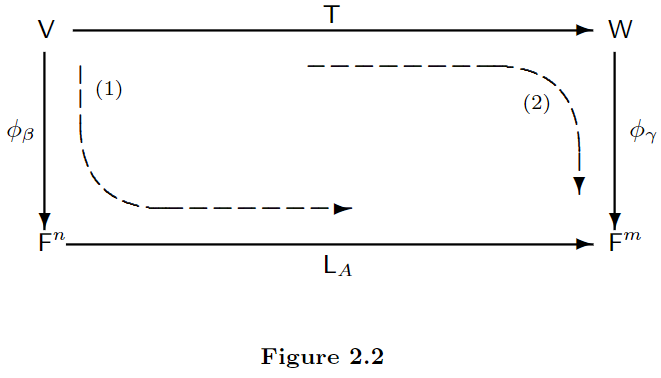
\includegraphics[scale=0.35]{figure}
\end{figure}

\begin{proof}
    We may write $\mathsf{L}_A = \phi_{\gamma}\mathsf{T}\phi_{\beta}^{-1}$, since $\phi_{\beta}$ is an isomorphism. Then $\mathsf{R}(\mathsf{L}_A) = \mathsf{R}(\phi_{\gamma}\mathsf{T}\phi_{\beta}^{-1}) = \phi_{\gamma}\mathsf{T}\phi_{\beta}^{-1}(\mathbb{F}^n) = \phi_{\gamma}\mathsf{T}(\mathsf{V}) = \phi_{\gamma}\mathsf{R}(\mathsf{T})$. Since $\phi_{\gamma}$ is an isomorphism, $\mathsf{R}(\mathsf{L}_A)$ is a subspace of $\mathbb{F}^m$, and $\mathsf{R(T)}$ is a subspace of $\mathsf{W}$, then $\dim(\mathsf{R}(\mathsf{L}_A)) = \dim(\mathsf{R(T)})$. Thus $\rank(\mathsf{L}_A)=  \rank(\mathsf{T})$, and so in view of the equations $\dim(\mathbb{F}^n) = \nullity(\mathsf{L}_A) + \rank(\mathsf{L}_A) = \dim(\mathsf{V}) = \nullity(\mathsf{T}) + \rank(\mathsf{T})$ which come from the dimension theorem, $\rank(\mathsf{T}) = \rank(\mathsf{L}_A)$ and that $\nullity(\mathsf{T}) = \nullity(\mathsf{L}_A)$ fall out instantly. 
\end{proof}

\end{document}